
%%%%%%%%%%%%%%%%%%%%%%%%%%%%%%%%%%%%%
% [x] Removed we
% [x] Tidied up language


\paragraph{Roofline Analysis}
One method that can be used to evaluate the performance of the program is to use a roofline model. This requires calculating some metrics of the device being used - NVIDIA Tesla P100. It has a Peak TFLOP/s of 9.7 and a peak memory bandwidth of 730 GB/s. This allows the Operational Intensity of the ridge point to be calcualted as 13.3 = 9700/730. This can be used to decide if the program is memory or compute bound.

\begin{figure}[ht]
% This file was created by tikzplotlib v0.9.1.
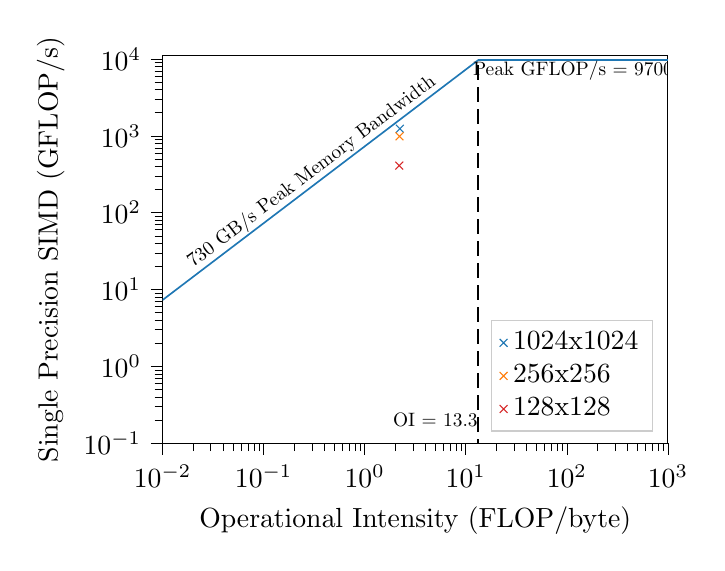
\begin{tikzpicture}

\definecolor{color0}{rgb}{0.12156862745098,0.466666666666667,0.705882352941177}
\definecolor{color1}{rgb}{1,0.498039215686275,0.0549019607843137}
\definecolor{color2}{rgb}{0.172549019607843,0.627450980392157,0.172549019607843}
\definecolor{color3}{rgb}{0.83921568627451,0.152941176470588,0.156862745098039}

\begin{axis}[
height=6.5cm,
width=8cm,
legend cell align={left},
legend style={fill opacity=0.8, draw opacity=1, text opacity=1, at={(0.97,0.03)}, anchor=south east, draw=white!80!black},
log basis x={10},
log basis y={10},
tick align=outside,
tick pos=left,
x grid style={white!69.0196078431373!black},
xlabel={Operational Intensity (FLOP/byte)},
xmin=0.01, xmax=1000,
xmode=log,
xtick style={color=black},
y grid style={white!69.0196078431373!black},
ylabel={Single Precision SIMD (GFLOP/s)},
ymin=0.1, ymax=11000,
ymode=log,
ytick style={color=black}
]

% OIs
\path [draw=black, semithick, dash pattern=on 5.55pt off 2.4pt]
(axis cs:13.28,0.01)
--(axis cs:13.28,9700);

% Peak GFLOPS
\path [draw=color0, semithick]
(axis cs:13.28,9700)
--(axis cs:1000,9700);

% Points
\addplot [only marks, draw=none, mark=x, draw=color0, fill=color0, colormap/viridis]
table{%
x                      y
2.2268 1239.7
};
\addlegendentry{1024x1024}
\addplot [only marks, draw=none, mark=x, draw=color1, fill=color1, colormap/viridis]
table{%
x                      y
2.21 988.03
};
\addlegendentry{256x256}
% \addplot [only marks, draw=none, mark=x, draw=color2, fill=color2, colormap/viridis]
% table{%
% x                      y
% 1.645 566.645
% };
% \addlegendentry{128x256}
\addplot [only marks, draw=none, mark=x, draw=color3, fill=color3, colormap/viridis]
table{%
x                      y
2.20 410.637
};
\addlegendentry{128x128}

\addplot [semithick, color0]
table {%
0.01 7.3
13.28 9700
};


% Numbers...
\draw (axis cs:115,7100) node[
  scale=0.7,
  text=black,
  rotate=0.0
]{Peak GFLOP/s = 9700};

\draw (axis cs:5,0.2) node[
  scale=0.7,
  text=black,
  rotate=0.0
]{OI = 13.3};

\draw (axis cs:0.3,340) node[
  scale=0.7,
  text=black,
  rotate=37.1
]{730 GB/s Peak Memory Bandwidth};

\end{axis}

\end{tikzpicture}

\vspace{-3mm}
\caption{Roofline model of NVIDIA Tesla P100}
\label{graph:roofline}
\vspace{-4mm}
\end{figure}

Using Oclgrind to measure the instructions used inside the kernels for a single iteration, some metrics can be calculated about the program. Each iteration of the 128x128 sized board load/stores 1206896 bytes and uses 2658888 floating point operations. 


This gives an operational intensity of 2.20. Therefore the program is memory bound, which would be expected of a lattice type program. The FLOP/s for the program can be calculated using the following formula: $Achieved\ FLOP/s = \frac{FLOPs\ per\ iteration * Iterations}{Runtime}$. This gives 410.6 GFLOP/s. This can be repeated for the other sizes.




Figure \ref{graph:roofline}, shows the four sizes performance on the roofline model. The 1024x1024 and 256x256 grids both achieved over 60\% peak memory bandwidth. They achieved bandwidths of 511.9 GB/s and 443.5 GB/s respectively. The 128x128 grid however has a significantly lower achieved bandwidth of just 186.6 GB/s. It could be possible that the previous effect of slow host code is occurring here as well. 
